% 
% $Author: awl8049 $ 
% $Date: 2010/09/06 18:18:28 $ 
% $Revision: 1.19 $
%
\documentclass[times,10pt,finalversion]{usetex-v1} 
\usepackage[nocompress]{cite}
\usepackage[pdftex]{graphicx} 
\DeclareGraphicsExtensions{.png,.jpg,.pdf}
\graphicspath{{graphics/}}
\usepackage[cmex10]{amsmath} 
\interdisplaylinepenalty=2500
\usepackage{array} 
\usepackage{booktabs}
\usepackage{url} 
\usepackage{setspace}
\usepackage[caption=false,labelfont=sf,textfont=sf,captionskip=5pt]{subfig}
\usepackage{fixltx2e}
\usepackage{dblfloatfix}
\usepackage[small]{caption}
% Variables and various other trickery to make the IEEE template
% behave.
\renewcommand{\figurename}{Fig.}
\usepackage{bibspacing}
\setlength{\bibspacing}{\baselineskip}
\usepackage{flushend}
% Now we putz around with things to try to squeeze things
% into the page limit
% First step-The basic stuff
% Some serious hacking redefines, may cause USENIX editors to complain
\setlength{\textheight}{9.45in}
\setlength{\textwidth}{6.95in}
\setlength{\marginparwidth}{0.0in}
\setlength{\tabcolsep}{3pt} 
\setlength{\parskip}{0pt}
\setlength{\parsep}{0pt}
\setlength{\headsep}{0pt}
\setlength{\topskip}{0pt}
\setlength{\topmargin}{0pt}
\setlength{\topsep}{0pt}
\setlength{\partopsep}{0pt}
\setlength{\abovedisplayskip}{0pt plus 0pt minus 0pt}
\setlength{\belowdisplayskip}{0pt plus 0pt minus 0pt}
 \renewcommand{\topfraction}{0.85}
 \renewcommand{\textfraction}{0.1}
 \renewcommand{\floatpagefraction}{0.75}
%\raggedbottom
\hyphenation{op-tical net-works semi-conductor} 
\pagestyle{empty}
\begin{document} 
\title{Chaotic Attractor Prediction for Server Run-time Energy
  Consumption} 
\author{
  \authname{Adam Lewis, Jim Simon, and Nian-Feng Tzeng}
  \authaddr{Center for Advanced Computer Studies, University
    of Louisiana, Lafayette, Louisiana 70504}
  \authurl{\url{{awlewis,jks1870,tzeng}@cacs.louisiana.edu}} }
\maketitle 
\thispagestyle{empty}
\begin{abstract}
\begin{small}
  This paper proposes a chaotic time series model of server system-wide
  energy consumption to capture the dynamics present in observed sensor
  readings of underlying physical systems.  Based on the chaotic model,
  we have developed a real-time predictor that estimates actual server
  energy consumption according to its overall thermal envelope.  This
  chaotic time series regression model relates processor power, bus
  activity, and system ambient temperatures for real-time prediction of
  power consumption during job execution to enable run-time control of
  their thermal impacts. An experimental case study compares our Chaotic
  Attractor Predictor (CAP) against previous prediction models
  constructed according to other statistical methods.
  Our CAP is found to be accurate within an average error of
  2\% (or 7\%) and the worst case error of 7\% (or 20\%) for the AMD Opteron
  processor (or for the Intel Nehalem processor), based on executing a
  set of SPEC CPU2006 benchmarks.
\end{small}
\end{abstract}
\section{Introduction}
\label{sec:Introduction}
Pro-active techniques for thermal management minimize server energy
consumption by adjusting the allocation of thread groups in a server to
available cores so as to consume the least amount of energy by all
thread groups. High-performance computing workloads result in the server
being fully utilized with little resources available for reactive
scheduling.  Effective adjustment of the resource allocation depends
upon predicting changes in temperature with reasonable accuracy, given
fluctuations in the system workload.  The interactions among many
subsystems within a server blade require the use of full-system models
that consider the thermal load of all components in a system. Thus, it
is critical to quantitatively understand the relationship among
thermal load, system utilization, and power consumption at the system
level so as to best optimize the scheduling of workloads.

Time series models operate by observing past outcomes of a physical
phenomenon so as to anticipate future values of that phenomenon; such models
are concerned more with the behavior of a phenomenon than
with how or why the phenomenon changes.  Many time series-based models
of processor energy consumption have been proposed
\cite{Rivoire2008}~\cite{Bhattacharjee2009}~\cite{Reich2010}; recent
work extends such models into the thermal domain \cite{Coskun2008}.
However, energy consumption, ambient temperature, and processor die
temperatures in servers can be affected by more than just past values
of those measurements made in isolation from each other.  Taking these
interactions into account requires the application of multivariate time
series.

Multivariate time series are typically handled in three broad classes of
mechanisms: auto-regressive, integrated, and moving average models
\cite{Box1994}.  Each of these classes assumes a linear relationship
between the dependent variable(s) and previous data points.  However, we
show through our analysis of experimental measurements of key processor
metrics (i.e., sensor readings) that the assumption of linearity does not
apply in all cases. Furthermore, our analysis indicates that the
non-linear behavior of these series is \textit{chaotic in nature}.
It thus leads to our development of a Chaotic Attractor Predictor (CAP).

In summary, the contributions of this work are three-fold. (1) We show, by
analyzing measurements from two different server systems, that server
energy consumption exhibits non-linear time series possessing chaotic
behavior, (2) we construct a model of server energy consumption using a
technique for analyzing chaotic time series of sensor measurements
during job execution, (3) we use measurements of server energy
consumption on two different server systems to compare the performance
of our model against those based on linear regression and
auto-regressive techniques.
\section{Background and Prior Work}
\label{sec:priorwork}
An analytical model of server energy consumption was built earlier
\cite{Lewis2008} by modeling energy consumption as a function of the
work done by the system in executing its computational tasks and of
residual thermal energy given off by the system in doing that work.  The
resulting dynamic system consumes energy expressed in the time domain as
follows:
\begin{small}
{\setlength{\abovedisplayskip}{2pt plus 2pt minus 2pt}
 \setlength{\belowdisplayskip}{2pt plus 2pt minus 2pt}
\begin{align}
  \label{eq:system}
  E_{system}&=\frac{d{P_{system}}}{d{t}}\nonumber\\
           &=f(E_{proc},E_{mem},E_{em},E_{board},E_{hdd})
\end{align}
}
\end{small}
where each of the terms in the above equation is defined as: (1)
$E_{proc}$: energy consumed in the processor due to computations, (2)
$E_{mem}$: energy consumed in the DDR SDRAM chips, (3) $E_{em}$: energy taken by the
electromechanical components in the system, (4) $E_{board}$:
energy consumed by peripherals that support the operation of the board,
and (5) $E_{hdd}$: energy consumed by the hard disk
drive during the system's operation.

We can approximate an energy consumption solution for this system by
considering (1) an initial energy state $E_{system}$ at time $t=0$ and
(2) a set of physical predictors that approximate the values of
$E_{proc}$, $E_{mem}$, $E_{board}$, and $E_{hdd}$ at the next interval
$t+\Delta t$.  The result is a time series
\begin{small}
{\setlength{\abovedisplayskip}{2pt plus 2pt minus 2pt}
 \setlength{\belowdisplayskip}{2pt plus 2pt minus 2pt}
\begin{equation}
\label{eq:tseries}
e\_sys=\hat{f}(e\_proc_{t},e\_mem_{t},e\_em_{t},e\_board_{t},e\_hdd_{t})
\end{equation}
}\end{small}
where each of quantities $e$ corresponds to one or more physically
observable predictors of the quantities in Eq.~(\ref{eq:system}). The
function $\hat{f}$ captures the method used to combine the physical
observations into $e\_sys$.  We place two key requirements upon
$\hat{f}$: (1) it must quickly compute estimates to be suitable for
real-time prediction of energy and temperature changes, and (2) it must
approximate the behavior of the original function $f$ to an acceptable
accuracy.  Our problem now becomes what shall we use in our predictor to
implement the $\hat{f}$ function?

A common approach for selecting predictors is to apply a linear
auto-regressive (AR) combination of CPU utilization, disk-utilization,
and hardware performance counters as estimators for the quantities in
Eq.~(\ref{eq:tseries}).  Linear regressions model the relationship
between one or more variables, such that the model depends linearly on
unknown parameters to be estimated from a set of data.  An excellent
summary of models of this type can be found in \cite{Rivoire2008}, with
recent representative examples described in \cite{Lewis2008},
\cite{Bhattacharjee2009}, and \cite{Reich2010}.

Other global auto-regressive techniques have been proposed for both
energy and thermal modeling.  For example, Coskun \textit{et~al.}
\cite{Coskun2008} proposed the use of an Auto-Regressive Moving Average
(ARMA) technique as a means to model changes in temperature as part of a
thermally aware process scheduler.  An ARMA predictor makes estimates of
future values of a system by using past values. The ARMA model
assumes that the process is a stationary stochastic process. In a
stationary process, the probability distribution does not change with
time. As a result, neither the mean nor the variance will change over
time.  ARMA predictors are not suited for data that exhibits sudden
bursts of a large amplitude at irregular time epochs due to their
underlying assumptions of normality \cite{Tong1993}. This issue can be
addressed by corrective mechanisms that adapt the predictor to the
workload-related changes in a dynamic system.  For example,
Coskun~\textit{et~al.}\cite{Coskun2008} addressed this issue by
including a machine-learning based corrector that monitored workload
changes and adjusted the parameters of their ARMA model.

Another approach to dealing with this problem is the use of an adaptive
nonparametric regression scheme based upon partitioning the underlying
time series.  Multivariate Adaptive Regression Splines (MARS),
introduced by Friedman \cite{Friedman1991}, is an adaptive procedure
that addresses non-linearity by fitting a weighted sum of basis
functions to the data set, with the basis functions in three possible forms:
(1) a constant value of 1 that represents the intercept term of the
regression, (2) a hinge function of the form $max(0,x-c)$ or
$max(0,c-x)$ that represents knots in the regression, or (3) a product
of two or more hinge functions that model interactions between two or
more variables.  The selection of weights and hinge constants is
performed by a two-pass algorithm, with its forward pass adding basis
functions to the regression in an attempt to reduce the mean square
error while attempting to improve the model in its backwards pass by
removing terms based upon cross validation.
\begin{small}
{\setlength{\abovedisplayskip}{0pt plus 0pt minus 0pt}
 \setlength{\belowdisplayskip}{0pt plus 0pt minus 0pt}
\begin{table*}[tbp]
  \centering
    \caption{Model errors for AR, MARS, and CAP on AMD Opteron server}
    \label{tab:modelerroropt}
    \begin{tabular}[phtb]{c |r r c|r r c|r r c}
      \hline
      \multicolumn{1}{c|}{}&\multicolumn{3}{c|}{\small{\textbf{AR}}}&\multicolumn{3}{c|}{\small{\textbf{MARS}}}&\multicolumn{3}{c}{\small{\textbf{CAP}
          (with $n=5$,
            $p=200$, $r=16$)}}\\
        \hline
  &\multicolumn{1}{c}{\small{\textbf{Avg}}}&\multicolumn{1}{c}{\small{\textbf{Max}}}&\multicolumn{1}{c|}{\small{\textbf{RMSE}}}&\multicolumn{1}{c}{\small{\textbf{Avg}}}&\multicolumn{1}{c}{\small{\textbf{Max}}}&\multicolumn{1}{c|}{\small{\textbf{RMSE}}}&\multicolumn{1}{c}{\small{\textbf{Avg}}}&\multicolumn{1}{c}{\small{\textbf{Max}}}&\multicolumn{1}{c}{\small{\textbf{RMSE}}}\\
\multicolumn{1}{c|}{\small{\textbf{Benchmark}}}&\multicolumn{1}{c}{\small{\textbf{Err \%}}}&\multicolumn{1}{c}{\small{\textbf{Err \%}}}&\multicolumn{1}{c|}{}&\multicolumn{1}{c}{\small{\textbf{Err \%}}}&\multicolumn{1}{c}{\small{\textbf{Err \%}}}&\multicolumn{1}{c|}{\small{\textbf{}}}&\multicolumn{1}{c}{\small{\textbf{Err \%}}}&\multicolumn{1}{c}{\small{\textbf{Err \%}}}&\multicolumn{1}{c}{}\\
      \hline      
      \small{astar }&\small{3.1\%}&\small{8.9\%}&\small{2.26}&\small{2.5\%}&\small{9.3\%}&\small{2.12}&\small{0.9\%}&\small{5.5\%}&\small{0.72}\\
      \small{games }&\small{2.2\%}&\small{9.3\%}&\small{2.06}&\small{3.0\%}&\small{9.7\%}&\small{2.44}&\small{1.0\%}&\small{6.8\%}&\small{2.06}\\
      \small{gobmk }&\small{1.7\%}&\small{9.0\%}&\small{2.30}&\small{3.0\%}&\small{9.1\%}&\small{2.36}&\small{1.6\%}&\small{5.9\%}&\small{2.30}\\
      \small{zeusmp}&\small{2.8\%}&\small{8.1\%}&\small{2.14}&\small{2.8\%}&\small{7.9\%}&\small{2.34}&\small{1.0\%}&\small{5.6\%}&\small{2.14}\\
      \hline
    \end{tabular}
  \end{table*}
}
\end{small}
\begin{small}
{\setlength{\abovedisplayskip}{0pt plus 0pt minus 0pt}
 \setlength{\belowdisplayskip}{0pt plus 0pt minus 0pt}
\begin{table*}[tbp]
  \centering
    \caption{Model errors for AR, MARS, and CAP on Intel Nehalem server}
    \label{tab:modelerroroptIntel}
    \begin{tabular}[phtb]{c |r r c|r r c|r r c}
      \hline
      \multicolumn{1}{c|}{}&\multicolumn{3}{c|}{\small{\textbf{AR}}}&\multicolumn{3}{c|}{\small{\textbf{MARS}}}&\multicolumn{3}{c}{\small{\textbf{CAP} (with $n=5$,
            $p=200$, $r=18$)}}\\
        \hline
  &\multicolumn{1}{c}{\small{\textbf{Avg}}}&\multicolumn{1}{c}{\small{\textbf{Max}}}&\multicolumn{1}{c|}{\small{\textbf{RMSE}}}&\multicolumn{1}{c}{\small{\textbf{Avg}}}&\multicolumn{1}{c}{\small{\textbf{Max}}}&\multicolumn{1}{c|}{\small{\textbf{RMSE}}}&\multicolumn{1}{c}{\small{\textbf{Avg}}}&\multicolumn{1}{c}{\small{\textbf{Max}}}&\multicolumn{1}{c}{\small{\textbf{RMSE}}}\\
\multicolumn{1}{c|}{\small{\textbf{Benchmark}}}&\multicolumn{1}{c}{\small{\textbf{Err \%}}}&\multicolumn{1}{c}{\small{\textbf{Err \%}}}&\multicolumn{1}{c|}{}&\multicolumn{1}{c}{\small{\textbf{Err \%}}}&\multicolumn{1}{c}{\small{\textbf{Err \%}}}&\multicolumn{1}{c|}{\small{\textbf{}}}&\multicolumn{1}{c}{\small{\textbf{Err \%}}}&\multicolumn{1}{c}{\small{\textbf{Err \%}}}&\multicolumn{1}{c}{}\\
      \hline
      \small{astar }&\small{5.9\%}&\small{28.5\%}&\small{4.94}&\small{5.4\%}&\small{28.0\%}&\small{4.97}&\small{1.1\%}&\small{20.8\%}&\small{1.83}\\
      \small{games }&\small{5.6\%}&\small{44.3\%}&\small{5.54}&\small{4.7\%}&\small{33.0\%}&\small{4.58}&\small{1.0\%}&\small{14.8\%}&\small{1.54}\\
      \small{gobmk }&\small{5.3\%}&\small{27.8\%}&\small{4.83}&\small{4.1\%}&\small{27.9\%}&\small{4.73}&\small{1.0\%}&\small{21.5\%}&\small{2.13}\\
      \small{zeusmp}&\small{7.7\%}&\small{31.8\%}&\small{7.24}&\small{11.6\%}&\small{32.2\%}&\small{8.91}&\small{3.3\%}&\small{20.6\%}&\small{3.31}\\
      \hline
    \end{tabular}
  \end{table*}
}
\end{small}
\section{Linear Regression: AR and  MARS}
\label{sec:linear}
A set of experiments was carried out to evaluate the performance of
power models built using AR and MARS techniques to approximate a
solution for dynamic systems following Eq.~(\ref{eq:system}). Observable
predictors of system activity were chosen for each of the quantities in
Eq.~(\ref{eq:tseries}) under two test systems: (1) an Oracle/Sun x2200
(AMD Opteron) server and (2) a Dell PowerEdge R610 (Intel Xeon X5300
Nehalem) server.  AR and MARS models for Eq.~(\ref{eq:tseries})
were created from data collected by executing a set of high-performance
computing benchmarks from the SPEC CPU2006 benchmark suite: bzip2,
cactusadm, gromac, leslie3d, omnetpp, and perlbench
\cite{Spec2006}. These models were then used as a predictive tool for
another set of CPU2006 benchmarks (astar, gobmk, calculix, and zeusmp)
as a means of evaluating the predictive performance of each model.

The results under these linear regression techniques (AR and MARS) are
summarized in Tables~\ref{tab:modelerroropt} and
\ref{tab:modelerroroptIntel}. All three techniques predict well over the
long term, with an average error ranging between 1.7\% and 3.1\%
depending upon method and benchmark.  However, they suffer from poor
performance in the short term, with maximum errors ranging from 7.9\% to
9.3\% for the AMD Opteron server and in the range of 15\% and 44\% for
the Intel Nehalem server. An analysis of the power traces for the
different benchmarks reveals hints of this behavior.  Consider the power
trace shown in \figurename~\ref{fig:amdzeusmppwr} for the SPEC CPU2006
zeusmp benchmark executed on an AMD Opteron server.  We saw indications
of (1) periodic behavior throughout the length of the run and (2) large
swings in the power draw though the course of the benchmark run. Similar
behavior was observed for other benchmarks on both server systems.
Thus, it is reasonably conjectured that non-linear dynamics exist in the
two test systems.  Furthermore, the behavior of the power draw is such
that the linear regression-based predictors will occasionally
mis-predict by large amounts (up to 44\%, as indicated in
Table~\ref{tab:modelerroroptIntel}).  The physical behavior of the
system uncovers that such large swings in power draw cannot be
completely attributed to noise and, as result, we must account for them
within our model.
\begin{figure}[bthp]
      \centering
      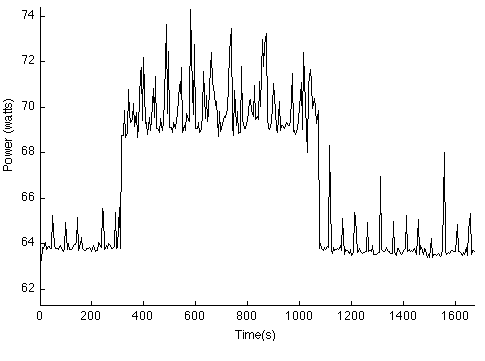
\includegraphics[width=3.4in,height=1.2in]{amdzeusmppwr2}
%      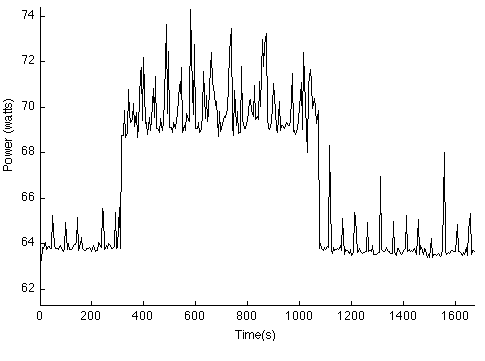
\includegraphics[scale=0.3]{amdzeusmppwr2}
      \caption{Power trace for zeusmp on AMD Opteron.}
      \label{fig:amdzeusmppwr}
\end{figure}
\section{Chaotic Behavior}
\label{sec:chaos}
We performed an analysis on the data collected from our test systems to
determine if the behavior of our time series can be attributed to a certain
form of chaotic behavior.  A chaotic process is one which is highly
sensitive to a set of initial conditions.  Small differences in those
initial conditions yield widely diverging outcomes in such chaotic
systems.  In order to determine whether a process is chaotic, we must be
able to show that it demonstrates high sensitivity to initial
conditions, topological mixing, and an indication that its periodic
orbits are dense \cite{Sprott2003}. After analyzing our experimental
data, we believe that the power consumption of a server demonstrates
chaotic behavior, as detailed next. 

In order to evaluate a server's sensitivity to initial conditions, we
consider the Lyapunov exponents of the time series data
observed while running those benchmarks described in the previous section.
The Lyapunov exponent quantifies the sensitivity of a system such that a
positive Lyapunov exponent indicates that the system is chaotic
\cite{Sprott2003}.  The average Lyapunov exponent can be calculated
using:
\begin{small}
{\setlength{\abovedisplayskip}{0pt plus 0pt minus 0pt}
 \setlength{\belowdisplayskip}{0pt plus 0pt minus 0pt}
  \begin{equation}
    \label{avgLypEq}
    \lambda =
    \lim_{N\to\infty}\frac{1}{N}\sum_{n=0}^{N-1}ln|f'(X_n)|.\nonumber
  \end{equation}
}
\end{small}
We found a positive Lyapunov exponent when performing this calculation
on our data set ranging from 0.01 to 0.28 (or 0.03 to 0.35) on the AMD
(or Intel) test server, as listed in Table~\ref{tab:chaotic},
where each pair indicates the parameter value of the AMD server followed by that of the Intel server.
Therefore, our data has met the first and the most significant criterion
to qualify as a chaotic process.

The second indication of the chaotic behavior of the time series in
Eq.~(\ref{eq:tseries}) is an estimate of the Hurst parameter $H$
for the data sets collected in each benchmark. 
A real number in the range of $(0,1)$, the Hurst parameter is in the exponents of the
covariance equation for Fractional Brown motion (fBm) \cite{Sprott2003}.
If the value of the Hurst parameter is greater than $0.5$, an
increment in the random process is positively correlated and
long range dependence exists in the case of time series.  In a
chaotic system, a value of $H$ approaching 1.0 indicates the presence of
self-similarity in the system.  As demonstrated in
Table~~\ref{tab:chaotic}, the time series data collected in our
experiments all have values of $H$ close to 1.0, ranging from 0.93 to
0.98 (or 0.93 to 0.97) on the AMD (or Intel) test server.
\begin{small}
  \begin{table}[bthp]
    \caption{Indications of chaotic behavior in power time series (AMD, Intel)}
    \label{tab:chaotic}  \centering
    \begin{tabular}{c | r r r }
      \hline
      \hline
      \multicolumn{1}{c |}{\small{\textbf{Benchmark}}}&\multicolumn{1}{c}{\small{\textbf{Hurst}}}&&\multicolumn{1}{c}{\textbf{\small{Average}}}\\
      \multicolumn{1}{c |}{~}&\multicolumn{1}{c}{\small{\small{\textbf{Parameter}}}}&&\multicolumn{1}{c}{\small{\textbf{Lyapunov}}}\\
      \multicolumn{1}{c |}{~}&\multicolumn{1}{c}{(\small{$H$)}}&&\multicolumn{1}{c}{\small{\textbf{Exponent}}}\\
      \hline
      \small{bzip2}&\small{(0.96, 0.93)}&&\small{(0.28, 0.35)}\\
      \small{cactusadm}&\small{(0.95, 0.97)}&&\small{(0.01, 0.04)}\\
      \small{gromac}&\small{(0.94, 0.95)}&&\small{(0.02, 0.03)}\\
      \small{leslie3d}&\small{(0.93, 0.94)}&&\small{(0.05, 0.11)}\\
      \small{omnetpp}&\small{(0.96, 0.97)}&&\small{(0.05, 0.06)}\\
      \small{perlbench}&\small{(0.98, 0.95)}&&\small{(0.06, 0.04)}\\
      \hline
      \hline
    \end{tabular}
  \end{table}
\end{small}
\begin{figure*}[!b]
  \begin{minipage}[b]{0.5\linewidth}
      \centering
      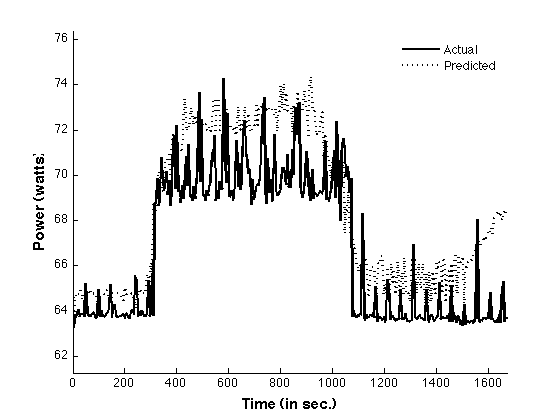
\includegraphics[width=1.0\linewidth,height=1.8in]{amdzeusmars}
%      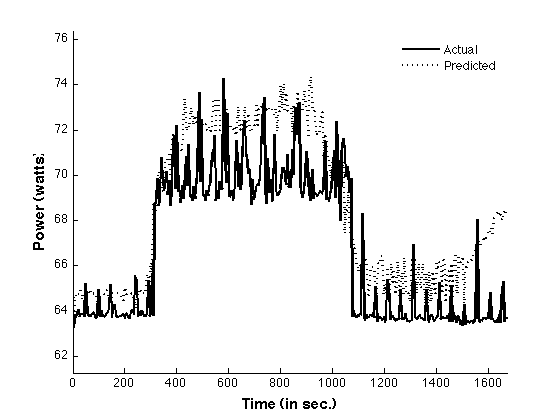
\includegraphics[scale=0.5]{amdzeusmars}
      \caption{Actual power results versus predicted results for zeusmp
        benchmark under MARS for AMD Opteron.}
      \label{fig:amdzeusmars}
  \end{minipage}\quad
  \begin{minipage}[b]{0.5\linewidth}
      \centering
      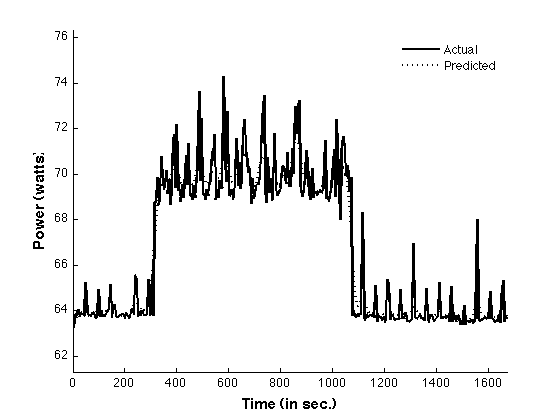
\includegraphics[width=1.0\linewidth,height=1.8in]{amdzeuspredict}
%      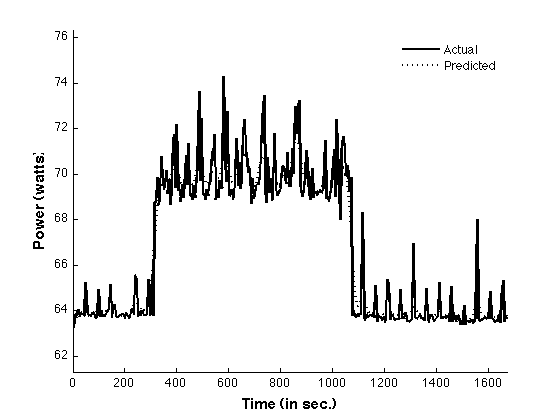
\includegraphics[scale=0.5]{amdzeuspredict}
      \caption{Actual power results versus predicted results for zeusmp
        benchmark under CAP for AMD Opteron.}
      \label{fig:amdzeuscapp}
  \end{minipage}
\end{figure*}
\section{Predicting from Chaos}
\label{sec:cappredict}
From a predictive standpoint, the unpredictable deterministic behavior
of chaotic time series means that it is difficult to build a predictor
that takes a global parametric view of the data in the series.  However,
it is possible to generate a highly accurate short-term prediction by
reconstructing the attractor in the phase space of the time series and
applying a certain form of least square prediction to the resulting vector
space \cite{Itoh1995}.
\subsection{Chaotic Predictor: CAP}
\label{sec:cap}
Given the time series introduced in Eq.~(\ref{eq:tseries}), we define
$X_{t}$ to be the value of $e_{system}$ at time $t$, and $r$ to be the
total number of sensors and OS measures to provide metric readings.
According to Taken's Delay Embedding Theorem \cite{Sprott2003}, there
exists a function $\hat{f}(X_{t})$ whose behavior in the phase space
reflects the behavior of the attractors in the original time series.
Our problem now becomes finding a means to approximate $\hat{f}$.

We introduce the concept of a Chaotic Attractor Predictor
(CAP) that defines $\hat{f}$ in terms of linear least squares
regression of a multivariate local polynomial of degree $r$.
Multivariate local linear regression is a common non-parametric
technique for time series approximations.  With CAP, we extend this
concept to predict the behavior of a chaotic time series by following
the approximation method proposed earlier \cite{Itoh1995}. CAP is a
predictor that exhibits the computational advantages of polynomial time
complexity while capturing the dynamics of test systems.

Let $x$ be an observation (involving $r$ metric readings) at some future
time $t+\Delta t$ and $X_{u}$ be a prior observation (involving $r$
metric readings) at time $u$ for $u=t-1,\dots,t-p$.  For CAP, we use the
standard d-variate normal density function, with $\|x\|$ being the norm
of vector $x$:
\begin{small}
{\setlength{\abovedisplayskip}{0pt plus 0pt minus 0pt}
 \setlength{\belowdisplayskip}{0pt plus 0pt minus 0pt}
  \begin{equation}
K(x)=(2\pi)^{-\frac{m}{2}}exp(-\|x\|^{2}/2)\nonumber
\end{equation}
}\end{small}
as a tool to localize the
neighborhood in which we define our polynomial.  We do this through
\textit{kernel weighting} with a defined bandwidth matrix $H$ for
localization by assigning a weight of $ K_{H}(x)=|H^{-1}|K(H^{-1}x)$.  This
can be simplified by taking the bandwidth matrix $H=hI_{r}$, with $h$
being a scalar value and $I_{r}$ being the identity matrix of order
$r$.

A local constant approximation for $\hat{f}$ is defined next
in terms of a locally weighted average \cite{Box1994} over
the next $n$ observations, based on the prior $p$ observations
of $X_{t-1}, \ldots, X_{t-p}$ (each with $r$ metric readings):
\begin{small}
{\setlength{\abovedisplayskip}{0pt plus 1pt minus 1pt}
 \setlength{\belowdisplayskip}{0pt plus 1pt minus 1pt}
  \begin{equation}
    \label{eq:localconst}
    \hat{f}(x)=\dfrac{\displaystyle\sum_{t=p+1}^{n+p}O_{p}*K_{H}(X_{t-1}-x)}{\displaystyle\sum_{t=p+1}^{n+p}K_{H}(X_{t-1}-x)}\nonumber
  \end{equation}
}
\end{small}
with $O_{p}=(X_{t-1},\ldots,X_{t-p})^{T}$.
 
\begin{figure*}[bth]
  \begin{minipage}[b]{0.5\linewidth}
    \centering
    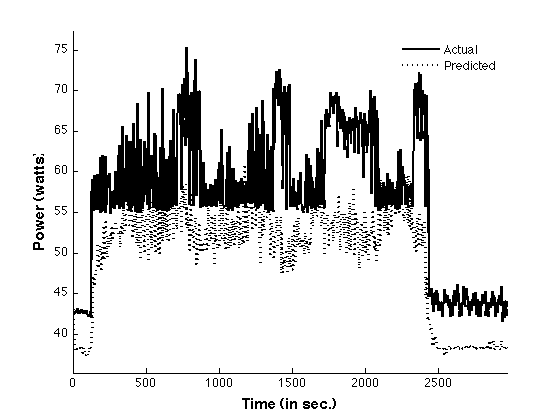
\includegraphics[width=1.0\linewidth,height=1.8in]{intelzeusmars}
%    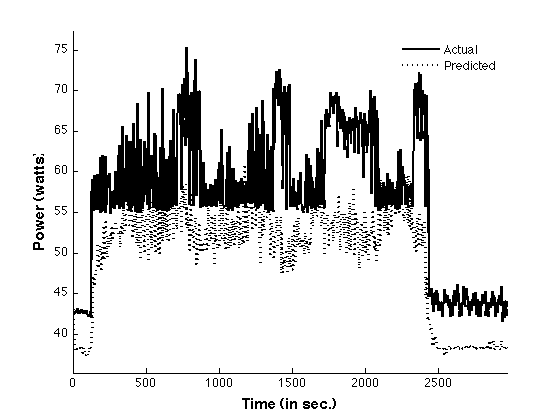
\includegraphics[scale=0.5]{intelzeusmars}
    \caption{Actual power results versus predicted results for zeusmp
      benchmark under MARS for Intel Nehalem.}
    \label{fig:intelzeusmars}
  \end{minipage}\quad
  \begin{minipage}[b]{0.5\linewidth}
    \centering
    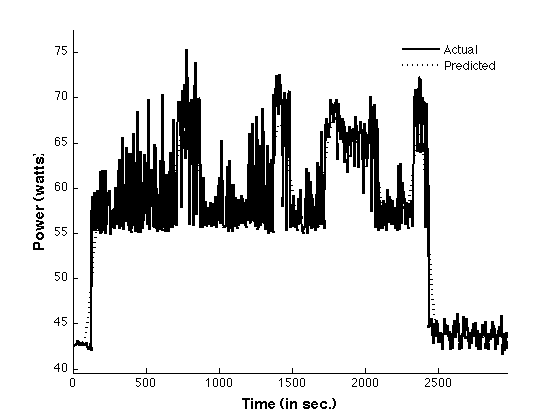
\includegraphics[width=1.0\linewidth,height=1.8in]{intelzeuspredict}
%    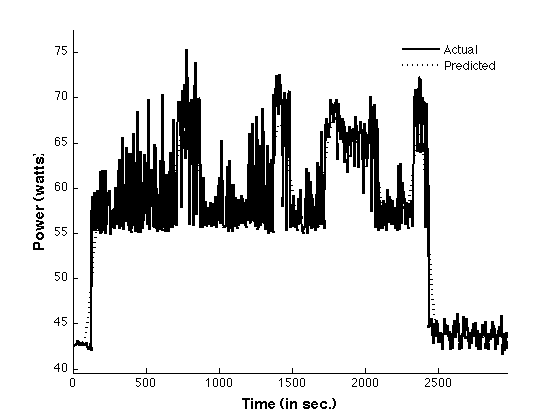
\includegraphics[scale=0.5]{intelzeuspredict}
    \caption{Actual power results versus predicted results for zeusmp
      benchmark under CAP for Intel Nehalem.}
    \label{fig:intelzeuspredict}
  \end{minipage}
\end{figure*}

The process can be improved by defining a local linear approximation
via applying a truncated Taylor series expansion of $\hat{f}$:
\begin{small}
{\setlength{\abovedisplayskip}{0pt plus 0pt minus 0pt}
 \setlength{\belowdisplayskip}{0pt plus 0pt minus 0pt}
  \begin{equation}
    \label{eq:localtaylor}
    \hat{f}(X)=\hat{f}(x)+\hat{f}^{'}(x)^{T}(X-x).\nonumber
  \end{equation}
}\end{small}
The coefficients of the polynomial $\hat{f}$ are then determined by minimizing
\begin{small}
{\setlength{\abovedisplayskip}{0pt plus 0pt minus 0pt}
 \setlength{\belowdisplayskip}{0pt plus 0pt minus 0pt}
  \begin{equation}
    \label{eq:lsq}
    \displaystyle\sum_{t=p+1}^{n+p}\left[X_{t}-a-b^{T}(X_{t-1}-x)\right]^{2}*K_{H}(X_{t-1}-x).
  \end{equation}
}\end{small}
with respect to $a$ and $b$, which are estimators to $\hat{f}(x)$ and
$\hat{f}'(x)$, respectively. The predictor generated by
solving Eq.~(\ref{eq:lsq}) can be explicitly written, according to \cite{Box1994}, as
\begin{small}
{\setlength{\abovedisplayskip}{0pt plus 1pt minus 1pt}
 \setlength{\belowdisplayskip}{0pt plus 1pt minus 1pt}
  \begin{equation}
    \label{eq:locallin}
    \hat{f}(x)=\frac{1}{n}\displaystyle\sum_{t=p+1}^{n+p}(s_{2}-s_{1}*(x-X_{t-1}))^{2}* K_{H}((x-X_{t-1})/h)
  \end{equation}
}\end{small}
with
$s_{i}=\frac{1}{n}\displaystyle\sum_{t=p+1}^{n+p}(x-X_{t-1})^{i}*K_{H}((x-X_{t-1})/h)$
for $i$ = 1 or 2.

There are three steps involved in the process of establishing a CAP
predictor: (1) creating a training set for the process, (2) using the
observations from the training set to find the appropriate delay
embedding using Takens Theorem and then apply the nearest neighbors
algorithm in the embedded set to identify the attractors, and (3)
solving the resulting linear least squares problem that arises from
applying Eq.~(\ref{eq:lsq}) to the attractors using the function
expressed by Eq.~(\ref{eq:locallin}). The time complexity of creating a
predictor is governed by the third step in the process.  The task of
reconstructing the state space by delay embedding is linear in time as
one must make up to $d$ passes through the observations, under the
embedding dimension of $d$.  Thus, the time required is $O(dn)$, where
$n$ is the number of next observations.  Then, it becomes a matter of
applying a naive form of $k$-th nearest neighbors algorithm to identify
the points in the attractors.  This step involves finding the squared
distance of all the points in the nearest analogs in the Takens set and
then sorting the result to determine the $d$-nearest neighbors.  This
step takes $O(n\log{n}+n)$.  We avoid the cost of computing the
linear least squares solution in the third step by using the explicit
expression given in Eq.~(\ref{eq:locallin}).
The time complexity of computing this expression can be shown to be $O(n*n)$,
with $O(n)$ due to computing $s_{i}$, for $i$ = 1 or 2.
As a result, the time complexity for establishing a CAP predictor
equals $O(n^{2})$.  It should be noted that
the construction of a CAP predictor is done only once for a given server,
irrespective of applications executed on the server.
\subsection{Evaluation and Results}
\label{sec:evaluation}
We evaluated the predictive performance of CAP versus linear regression
techniques by applying a local linear CAP to the same collected data
used in Section \ref{sec:linear}. The training set (bzip2, cactusadm,
gromac, leslie3d, omnetpp, perlbench \cite{Spec2006}) for the model was
created by taking the geometric mean of all the time series involved in
evaluating linear regression techniques. Next, the process described in
Section \ref{sec:cap} was employed to determine the attractors of the
resulting time series, followed by generating an approximating
polynomial to fit the attractor. The resulting predictor was applied to
those benchmarks (i.e., astar, gobmk, calculix, and zeusmp) used to
evaluate linear regression techniques. The results of this experiment
are summarized in Tables~\ref{tab:modelerroropt} and
\ref{tab:modelerroroptIntel} under the column ``CAP''. 
{\setlength{\abovedisplayskip}{0pt plus 0pt minus 0pt}
 \setlength{\belowdisplayskip}{0pt plus 0pt minus 0pt}
\begin{figure}[!h]
  \centering
  %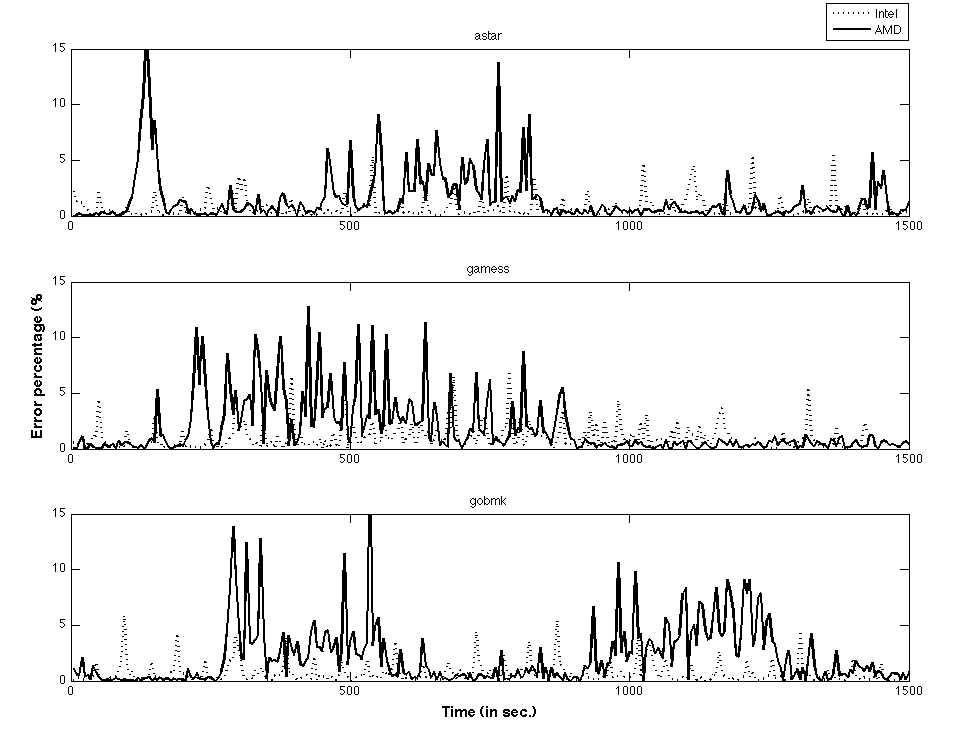
\includegraphics[width=1.0\linewidth,height=2.4in]{pcterr}
  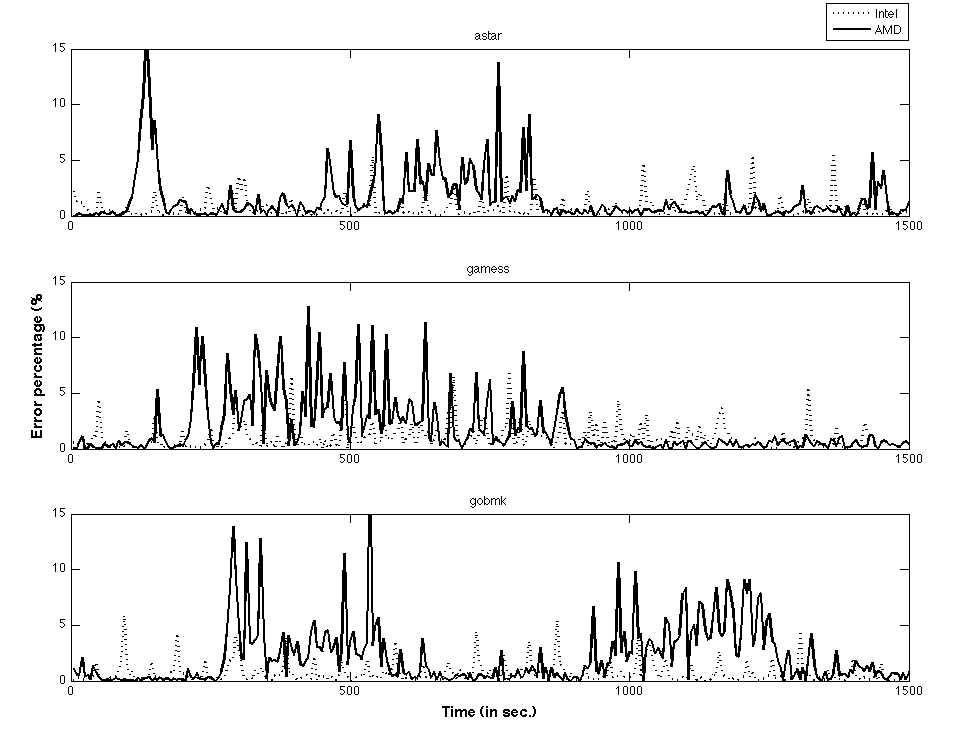
\includegraphics[scale=0.32]{pcterr}
  \caption{CAP error rates versus time for three other benchmarks.}
  \label{fig:pcterr}
\end{figure}} 

CAP predicts power changes in the long term with an average error in the
range from 1.0\% to 1.6\% for the AMD Opteron server and 1.4\% to 4.2\%
for the Intel server.  Maximum errors are far better under CAP than
under its linear regression counterparts, ranging from 5.5\% to 6.8\%
only for the AMD Opteron server, in contrast to as large as 9.7\% under
MARS.  Better prediction was observed similarly for the Intel server,
with the maximum error dropping to 21.5\% from 33.0\% under MARS,
accompanied by corresponding improvement in the Root Mean Square Error
(RMSE) for all benchmarks.  As expected, CAP provides a better fit
overall and at the start as well as the end of the series.  This
behavior, as opposed to a regression spline technique like MARS, results
from better prediction of piecewise local polynomials versus the
regression spline being global in nature. A detailed comparison between
MARS and CAP predictors for the AMD server can be seen in
\figurename~\ref{fig:amdzeusmars} and \figurename~\ref{fig:amdzeuscapp},
where $n=5$, $p=200$ and $r=16$. CAP exhibits far smaller difference
between actual and predicted power consumption amounts under the CPU2006
zeusmp benchmark.  Likewise, a contrast between MARS and CAP predictors
for the Intel server under the zeusmp benchmark is demonstrated in
\figurename~\ref{fig:intelzeusmars} and
\figurename~\ref{fig:intelzeuspredict}, where $n=5$, $p=200$ and $r=18$.
\figurename~\ref{fig:pcterr} illustrates the error rates for the other
three evaluated benchmarks over their execution intervals.  Those
benchmarks exhibit similar behavior to what is seen under the zeusmp
benchmark, shown in
Figs. \ref{fig:amdzeusmars}-\ref{fig:intelzeuspredict}.
\section{Conclusion}
\label{sec:conclusions}
In this paper, we have shown that models constructed from global
auto-regressive methods, such as AR, ARMA, and MARS, demonstrate
behavior that makes them problematic for predicting server energy
consumption.  The proposed CAP overcomes the limitations of the
previous linear regression-based methods by addressing the non-linear
aspects of the time series data while capturing the underlying chaotic
behavior of the dynamic physical system.  CAP involves $O(n\log{n})$
time complexity and requires no additional hardware beyond those made
available in recent processors, nor any tool outside those provided by
operating systems. As a result, CAP can support high-performance and
real-time application workloads, readily applicable for run-time energy
consumption prediction.  
\begin{small}
\section*{Acknowledgement}
This work was supported in part by the U.S. Department of Energy (DOE)
under Award Number DE-FG02-04ER46136 and by the Board of Regents, State
of Louisiana, under Contract Number DOE/LEQSF(2004-07)-ULL.
\end{small}
\label{sec:references} 
\begin{small}
\bibliographystyle{IEEEtran}
  \bibliography{timeseries.bib}
\end{small}
\end{document}


